\section*{Zadanie 7.}
\begin{task}
Dana jest linia współosiowa o średnicy $7\ mm$ i średnicy wewnętrznej $3\ mm$ wykonana z miedzi o przewodności właściwej równej $5*10^{7}\ \cfrac{S}{m}$ i wypełniona dielektrykiem o przenikalności właściwej 2.00 i tangensie kąta stratności równym 0.002. Obliczyć parametry jednostkowe linii ($L_{1},\ C_{1},\ G_{1},\ R_{1}$) dla częstotliwości $1GHz$. Które (czy też który) z parametrów będzie wyraźnie różny dla częstotliwości $10GHz$. Ile razy stłumi się moc fali w tej linii na odcinku 10 m (dla $1\ GHz$ i dla $10\ GHz$).\\
\end{task}

\begin{solution}
\begin{center}
$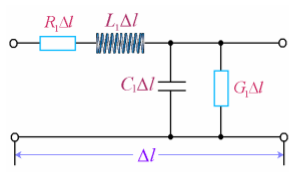
\includegraphics[scale=1]{7_1}$\\
\end{center}

$$L_{1}=\cfrac{\mu}{2\pi}\ln{\cfrac{a}{b}}=0.17\big{[}\cfrac{\mu H}{m}\big{]}$$
$$C_{1}=\cfrac{2\pi\epsilon}{\ln{\cfrac{a}{b}}}=0.13\big{[}\cfrac{nF}{m}\big{]}$$
$$\tg{\delta}=\cfrac{\sigma}{\omega\epsilon}=\cfrac{G_{1}}{\omega C_{1}} \ \ \implies \ G_{1}=\omega C_{1}\tg{\delta} = 0.82\big{[}\cfrac{mS}{m}\big{]}$$
$$\delta_{w}=\cfrac{2}{\sqrt{\omega\mu\sigma}}=2.25 \big{[}\mu m\big{]}$$
$$R=\cfrac{l}{\sigma S}\stackrel{l=1}{=}\cfrac{1}{\sigma S}\ \ \ S_{a}=2\pi a\delta_{w}\ \ \ S_{b}=2\pi b\delta_{w}$$
$$R_{1}=\cfrac{1}{ \sigma_{m}2 \pi a \detla_{w}}+\cfrac{1}{ \sigma_{m} 2 \pi \delta_{w}}=0.67 \big{[} \cfrac{\Omega}{m} \big{]}$$
$$\tg{\delta}=0.002=\cfrac{\sigma d}{\omega\epsilon}\ \ \implies \ \ \sigma d=\cfrac{4}{18}10^{-e}\big{[}\cfrac{S}{m}\big{]}$$
$$\alpha=\cfrac{\sigma d}{2}\sqrt{\cfrac{\mu}{\epsilon}}=\cfrac{10^{-3}}{9\sqrt{2}}$$
$$P(10m)=P(0)e^{-2\alpha 10m}\ \ \ \ \cfrac{P(10m)}{P(0m)}=e^{-2\alpha 10m}=0.553$$
\end{solution}
